\documentclass[a4paper,11pt,english]{article}
\usepackage[english]{babel} 
\usepackage[T1]{fontenc}    
\usepackage[utf8]{inputenc} 
\usepackage{graphicx}       
\usepackage{hyperref}      


\begin{document}

\title{Active strategies for object discovery}
\author{Phil Bradfield \and Jan Fabian Schmid}
	
\maketitle 

\section{Introduction}
Our project is to develop an autonomous mobile system for object detection.
Instead of using only single images to find positions and shapes of objects in an environment, we can use a sequence of images from different viewpoints.
It is desirable for an autonomous robot that he is able to interact and use objects in his environment. However, therefore he has to be aware of possible locations of objects, then he can try to classify objects.
For this task object detection can be used. An object detection algorithm would provide a list of object proposals that are worth to be analyzed in further detail.
Object proposals restrict the search space for useful objects.
Such restrictions are necessary, because every mobile system bears certain limitations to its capabilities. 
Mostly processing power, energy and time are limited.

Usually object detection algorithms only work on single 2D images \cite{atanasov2014nonmyopic}.
A mobile system, however, will produce a sequence of images during its process of exploring its environment.
This produces a number of additional challenges to the traditional 2D problem that we have to deal with.
One is that at each taken viewpoint a new set of object proposals is calculated, these have to be fused with previous object proposals. The second big problem is that the robot has to decide where to look next. Which is the problem of finding the Next Best View (NBV). 
For our project the goal is to analyze and evaluate multiple possible NBV-algorithms in their capability of finding good viewpoints to examine the environment.\medskip

This intermediate report is structured as follows:
The next subsection of this introductory chapter presents the three application scenarios that we want to test our system in.
Then some related work is described. The presented publications solved similar problems to the ones we encounter.
In chapter \ref{background} we will go into detail of some of the used approaches in our system.
Following, Chapter \ref{system} will provide an overview of the information flow in our system, some steps will be described in more detail. We also talk about the already done progress and about possible extensions to the system.
In the last Chapter \ref{timeline} we will try to assess in a timeline how we will proceed working on the system. 
 
\subsection{Application scenarios}
Currently three scenarios of application with different complexity are planned.
\begin{itemize}	
	\item \textbf{Table scenario}: Objects of different size, shape and color are assembled on a table. Some objects are partially or completely occluded by other objects, therefore a single viewpoint is not sufficient to detect all objects. The mobile system has a RGB-D camera mounted at an appropriate hight to look on the table. It can move freely around the table to reach different viewpoints.
	\item \textbf{Pre-recorded images scenario}: This scenario is only an intermediate application for testing during the development of the system. We utilize the same setting as in the table scenario, but without an autonomous system. Using a RGB-D camera on a tripod, we take pictures from different viewpoints of the table. The system can use these images for object detection, computation of a NBV or movement of the system is not required.
	\item \textbf{Scattered objects scenario}: For the most complex scenario objects lie scattered on the floor. The mobile system can move in between the objects to take views on different areas of the scene. This scenario is especially more demanding on the abilities of computing the NBV and moving the robot to the desired viewpoints, which should allow us to examine the pros and cons of different NBV-algorithms.
\end{itemize} 

\subsection{Related work}
In this chapter we introduce some other approaches in which subproblems we encounter ourself with our system have been solved.\medskip

García and Frintrop build a framework for 3D object detection by utilizing a visual attention system \cite{garcia2013computational}.
They work with a recorded video stream from an RGB-D camera. The color and depth stream are separately processed. 
The color stream is used to create so called proto-objects, which are areas with high probability of being part of an object. These proto-objects correspond to the peaks in the calculated saliency map. 
Simultaneously, the image is segmented into areas of pixel with similar color. 
For each proto-object the overlapping segments are considered to correspond to the proto-object. These segments are united to a object candidate.

At the same time, the depth stream is used to build a map of the scene.
By projecting the object candidates into the 3D map they are able to label voxels as associated to a certain object in the scene.
An inhibition of return (IOR) mechanism for three dimensional scenes is used to allow the algorithm to focus on one salient region after the other.

We can use this framework as a starting point for our project.
As the framework is used for pre-recorded videos, the active sensing part that we need is missing.
Apart from that, we can use the described methods for object candidate creation and the fusion of data from multiple views.
For our project it may not be necessary to implement a 3D IOR map. This is because we don't have to use a continuously moving video stream to find object candidates. In our case it is possible to stop movement at our desired viewpoints and take a picture from which object candidates are determined. \medskip

Meger et al. created with Curious George a mobile system that has been successful in the past in object recognition tasks \cite{meger2010curious}.
The robot is given a set of objects, it will then compute a visual classifier for each in a training phase.
Afterwards the robot drives autonomously through an environment. It is simultaneously exploring and searching for the known objects.
To build this map and navigate in it they have to solve the Simultaneous Localization and Mapping (SLAM) problem.
This is done with GMapping, which produces a 2D occupancy grid map from laser scan and odometry data (see Section \ref{system:slam}).
Curious George is analyzing his environment in two steps.
At first, the robot is guided through a frontier-based exploration algorithm, until a map of the whole scene is built.
Then, as a second phase, the scene is analyzed in more detail:
They use an attention system with a saliency map comparable to the one in the approach of García and Frintrop to find interesting places in the already discovered environment.
Saliency is used to focus the attention of the system to relevant parts of the environment. This is necessary as many possible views are redundant or promise only a very low information gain.
Therefore, visual saliency is used to evaluate the potential information gain of an area, supplementary the environmental structure is analyzed to find areas like desks where a high amount of objects is to be expected.

Even though the system of Meger et al. does object recognition, some parts of the system can be adopted by us.
We have to solve SLAM as well. Therefore, we will also use GMapping. Our robot has no laser range-finder to generate laser scan data, but with the depth data from Kinect we can simulate such data.
The two steps of exploring is an interesting approach that we can keep in mind for our system.
And as a first approach for a simple NBV-planner we could use a frontier-based exploration algorithm. \medskip

\section{Theoretical background}
\label{background}
\subsection{Saliency based object discovery}

\subsection{Fast SLAM}
\subsection{Surman approach}
\subsection{Subsumption architecture}

\section{System description and progress}
\label{system}
A general overview of our system is given in figure \ref{fig:overview}.

\begin{figure}
	\begin{center}
		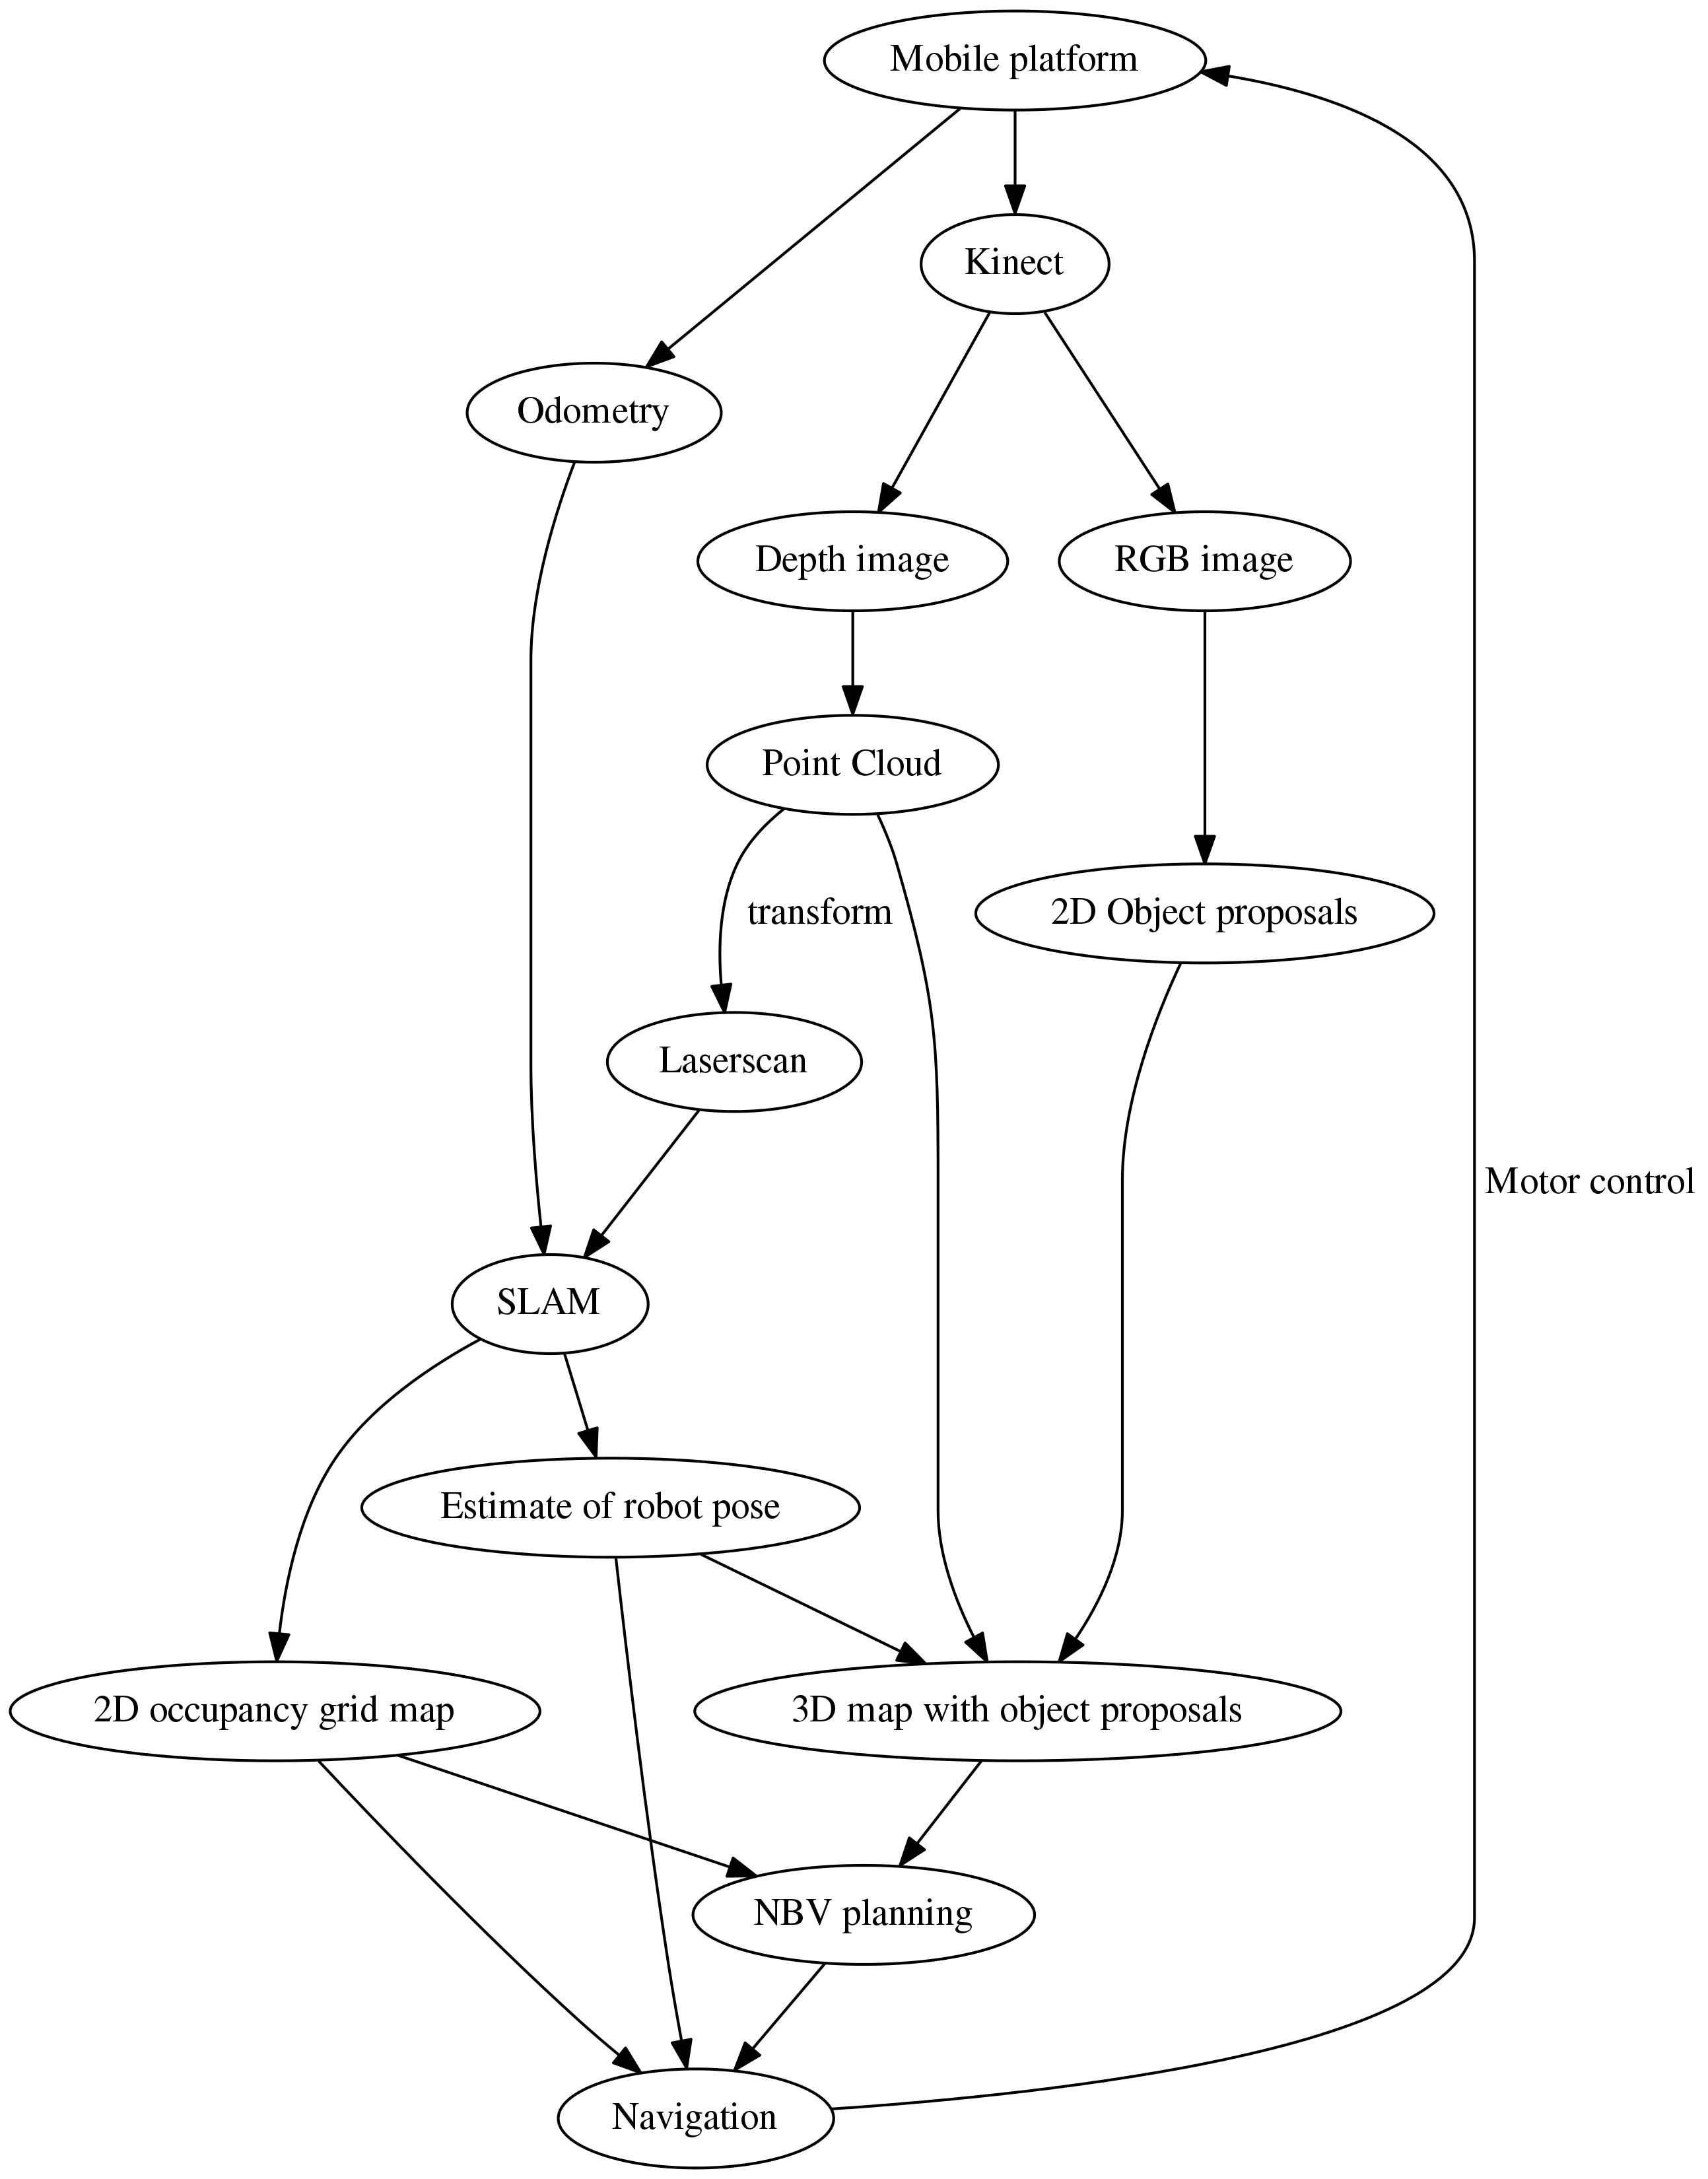
\includegraphics[width=1\linewidth]{dot/overview.png} 
		\caption{Overview of the system}
		\label{fig:overview}
	\end{center}
\end{figure}

Before we start explaining the graph in detail, it is useful to have a look at the available input and the desired output of our system.
\begin{itemize}
	\item \textbf{Input:}
	\begin{itemize}
		\item We will use a Turtlebot as mobile platform, which provides odometry data from the motion sensors.
		\item Onto the Turtlebot a Kinect is mounted, which provides RGB-D images of the scene.
	\end{itemize}
	\item \textbf{Output:}
	\begin{itemize}
		\item During operation of the system it is moving around the scene. Therefore, motor control can be seen as intermediate output of the system.
		\item The goal is to retrieve a 3D map with incorporated labels of all found object proposals.
	\end{itemize}  
\end{itemize}
Independent of the used application scenario the robot starts with no available knowledge of the scene.
Therefore, we are completely dependent on the system input to infer information.
At the beginning only a RGB-D image of the robot viewpoint at the start is available.

One processing line is now using the RGB image to find any possible objects in the view, this is described in detail in section \ref{system:obj_discovery}.
Simultaneously the depth image of the Kinect camera is processed.
The depth data is used to simulate a laser scanner, which provides depth data of one horizontal line in the robot view. 
This laser scan data is used together with the odometry data to solve the Simultaneous Localization And Mapping (SLAM) problem. This part is described in more detail in section \ref{system:slam}.
The SLAM-algorithm provides a 2D occupancy grid map, which is a kind of floor plan, containing information about obstacles and free space in the already discovered environment. A second output of SLAM is an estimate of the current robot pose.
This pose is used together with the new found object proposals of the current view and the current depth image to update the 3D map that contains a labeling of voxels to object proposals. This procedure is specified in section \ref{system:fusion}. 
The next step is to compute a next best viewpoint for the robot that should maximize the information gain about the environment.
For this computation all data that has been gathered to this point can be used, particularly the positions of already found object proposals and the current floor map will be used for this step. Details can be found in section \ref{system:nbv}.
Once a desired view point is calculated, it is used together with the current occupancy grid map and pose estimation to plan movement of the robot to this point in space.
This part is described in section \ref{system:navigation}.
The output of the navigation module is the motor control to move the system.
During movement the SLAM algorithm is constantly processing the camera data to update the map and keep track of the robot position.
Once the viewpoint is reached the next iteration of the described process is done.

After describing the individual parts of our system in more detail, the last subsection of this chapter provides a list of possible extensions to the system, that we will work on if time permits.
\subsection{Object discovery}
\label{system:obj_discovery}

\subsection{Solving SLAM}
\label{system:slam}
To solve the simultaneous localization and mapping we use a ROS wrapper for OpenSlam's GMapping algorithm, which is an implementation of Fast SLAM.
It uses laser scan and odometry data to compute a 2D occupancy grid map of the discovered environment.
The algorithm requires laser scan data of a horizontally-mounted laser range-finder.
We don't have such a laser range-finder; however, we can transform the depth image provided by the Kinect camera to such laser scan data.

The ROS wrapper provides topics to retrieve the build 2D occupancy map and the current pose estimation of the robot in this map.

\subsection{Fuse data of multiple views together}
\label{system:fusion}
\subsection{Determining the next best view}
\label{system:nbv}
\subsection{Navigation}
\label{system:navigation}
\subsection{Extensions}
\label{system:extensions}
In the following list we present possible extension to the core system that has been described so far in this chapter. 
The extensions could improve the system, but they shouldn't be essential for the performance of it.

\begin{itemize}
	\item Include depth information for the computation of object proposals.
	\item An additional NBV planning algorithm that exploits POMDPs.
\end{itemize}

\section{Timeline}
\label{timeline}

\newpage
\bibliographystyle{plain}
\addcontentsline{toc}{section}{Bibliography}% Add to the TOC
\bibliography{bib}

\end{document}
